\section{Text strings}

\subsection{\CCpp}

\label{C_strings}
The normal C strings are zero-terminated (\ac{ASCIIZ}-strings).

The reason why the C string format is as it is (zero-terminated) is apparently historical.
In [Dennis M. Ritchie, \IT{The Evolution of the Unix Time-sharing System}, (1979)]
we read:

\begin{framed}
\begin{quotation}
A minor difference was that the unit of I/O was the word, not the byte, because the PDP-7 was a word-addressed
machine. In practice this meant merely that all programs dealing with character streams ignored null
characters, because null was used to pad a file to an even number of characters.
\end{quotation}
\end{framed}

\myindex{Hiew}

In Hiew or FAR Manager these strings looks like this:

\begin{lstlisting}
int main()
{
	printf ("Hello, world!\n");
};
\end{lstlisting}

\begin{figure}[H]
\centering
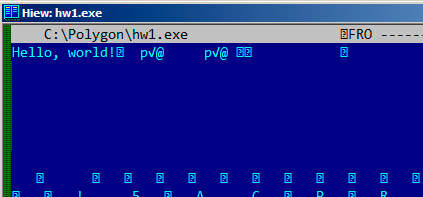
\includegraphics[scale=\NormalScale]{digging_into_code/strings/C-string.png}
\caption{Hiew}
\end{figure}

% FIXME видно \n в конце, потом пробел

\subsection{Borland Delphi}
\myindex{Pascal}
\myindex{Borland Delphi}

The string in Pascal and Borland Delphi is preceded by an 8-bit or 32-bit string length.

For example:

\begin{lstlisting}[caption=Delphi]
CODE:00518AC8                 dd 19h
CODE:00518ACC aLoading___Plea db 'Loading... , please wait.',0

...

CODE:00518AFC                 dd 10h
CODE:00518B00 aPreparingRun__ db 'Preparing run...',0
\end{lstlisting}

\subsection{Unicode}

\myindex{Unicode}

Often, what is called Unicode is a methods for encoding strings where each character occupies 2 bytes or 16 bits.
This is a common terminological mistake.
Unicode is a standard for assigning a number to each character in the many writing systems of the 
world, but does not describe the encoding method.

\myindex{UTF-8}
\myindex{UTF-16LE}
The most popular encoding methods are: UTF-8 (is widespread in Internet and *NIX systems) and UTF-16LE (is used in Windows).

\subsubsection{UTF-8}

\myindex{UTF-8}
UTF-8 is one of the most successful methods for
encoding characters.
All Latin symbols are encoded just like in ASCII,
and the symbols beyond the ASCII table are encoded using several bytes.
0 is encoded as
before, so all standard C string functions work with UTF-8 strings just like any other string.

Let's see how the symbols in various languages are encoded in UTF-8 and how it looks like in FAR, using the 437 codepage
\footnote{The example and translations was taken from here: 
\url{http://go.yurichev.com/17304}}:

\begin{figure}[H]
\centering
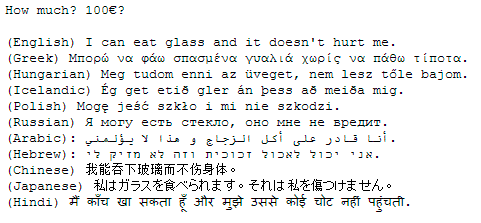
\includegraphics[scale=\NormalScale]{digging_into_code/strings/multilang_sampler.png}
\end{figure}

% FIXME: cut it
\begin{figure}[H]
\centering
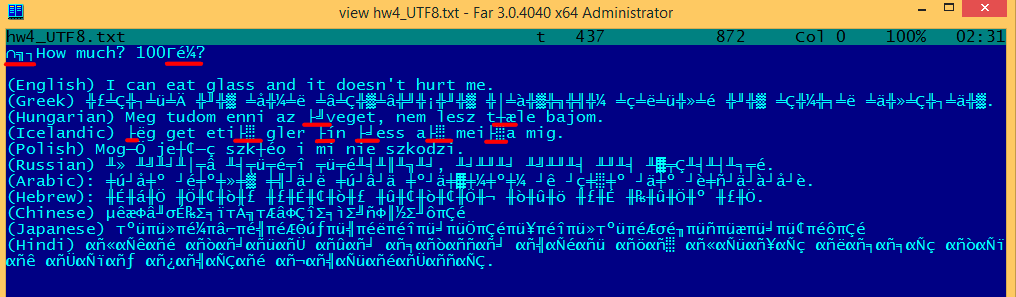
\includegraphics[scale=\FigScale]{digging_into_code/strings/multilang_sampler_UTF8.png}
\caption{FAR: UTF-8}
\end{figure}

As you can see, the English language string looks the same as it is in ASCII.

The Hungarian language uses some Latin symbols plus symbols with diacritic marks.

These symbols are encoded using several bytes, these are underscored with red.
It's the same story with the Icelandic and Polish languages.

There is also the \q{Euro} currency symbol at the start, which is encoded with 3 bytes.

The rest of the writing systems here have no connection with Latin.

At least in Russian, Arabic, Hebrew and Hindi we can see some recurring bytes, and that is not surprise:
all symbols from a writing system are usually located in the same Unicode table, so their code begins with
the same numbers.

At the beginning, before the \q{How much?} string we see 3 bytes, which are in fact the \ac{BOM}.
The \ac{BOM} defines the encoding system to be
used.

\subsubsection{UTF-16LE}

\myindex{UTF-16LE}
\myindex{Windows!Win32}
Many win32 functions in Windows have the suffixes \TT{-A} and \TT{-W}.
The first type of functions works
with normal strings, the other with UTF-16LE strings (\IT{wide}).

In the second case, each symbol is usually stored in a 16-bit value of type \IT{short}.

The Latin symbols in UTF-16 strings look in Hiew or FAR like they are interleaved with zero byte:

\begin{lstlisting}
int wmain()
{
	wprintf (L"Hello, world!\n");
};
\end{lstlisting}

\begin{figure}[H]
\centering
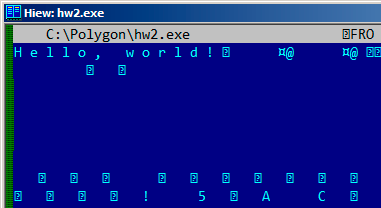
\includegraphics[scale=\NormalScale]{digging_into_code/strings/UTF16-string.png}
\caption{Hiew}
\end{figure}

We can see this often in \gls{Windows NT} system files:

\begin{figure}[H]
\centering
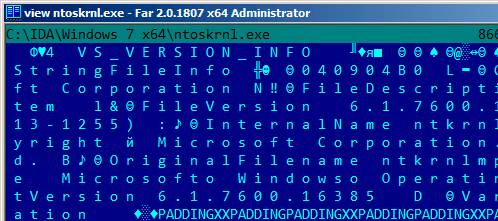
\includegraphics[scale=\NormalScale]{digging_into_code/strings/ntoskrnl_UTF16.png}
\caption{Hiew}
\end{figure}

\myindex{IDA}
Strings with characters that occupy exactly 2 bytes are called \q{Unicode} in \IDA:

\begin{lstlisting}
.data:0040E000 aHelloWorld:
.data:0040E000                 unicode 0, <Hello, world!>
.data:0040E000                 dw 0Ah, 0
\end{lstlisting}

Here is how the Russian language string is encoded in UTF-16LE:

\begin{figure}[H]
\centering
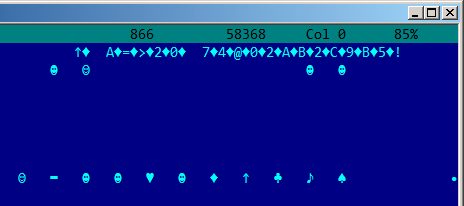
\includegraphics[scale=\NormalScale]{digging_into_code/strings/russian_UTF16.png}
\caption{Hiew: UTF-16LE}
\end{figure}

What we can easily spot is that the symbols are interleaved by the diamond character (which has the ASCII code of 4).
Indeed, the Cyrillic symbols are located in the fourth Unicode plane
\footnote{\href{http://go.yurichev.com/17003}{wikipedia}}.
Hence, all Cyrillic symbols in UTF-16LE are located in the \TT{0x400-0x4FF} range.

Let's go back to the example with the string written in multiple languages.
Here is how it looks like in UTF-16LE.

% FIXME: cut it
\begin{figure}[H]
\centering
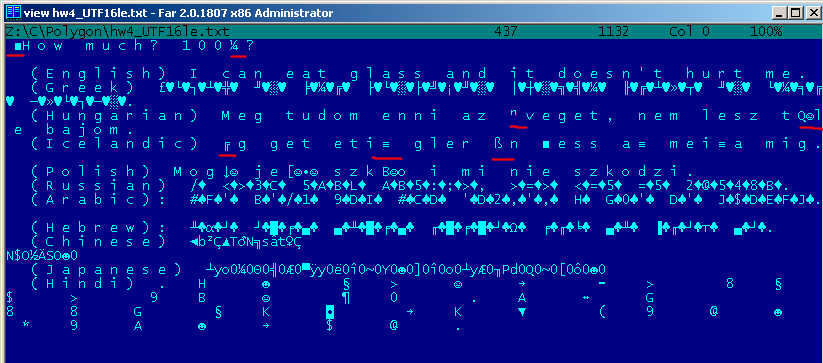
\includegraphics[scale=\FigScale]{digging_into_code/strings/multilang_sampler_UTF16.png}
\caption{FAR: UTF-16LE}
\end{figure}

Here we can also see the \ac{BOM} in the beginning.
All Latin characters are interleaved with a zero byte.

Some characters with diacritic marks (Hungarian and Icelandic languages) are also underscored in red.

% TODO: strings *NIX utility. procmonitor also shows strings...

\subsection{Base64}
\myindex{Base64}

The base64 encoding is highly popular for the cases when you need to transfer binary data as a text string.

In essence, this algorithm encodes 3 binary bytes into 4 printable characters:
all 26 Latin letters (both lower and upper case), digits, plus sign (\q{+}) and slash sign (\q{/}),
64 characters in total.

One distinctive feature of base64 strings is that they often (but not always) ends with 1 or 2 \gls{padding}
equality symbol(s) (\q{=}), for example:

\begin{lstlisting}
AVjbbVSVfcUMu1xvjaMgjNtueRwBbxnyJw8dpGnLW8ZW8aKG3v4Y0icuQT+qEJAp9lAOuWs=
\end{lstlisting}

\begin{lstlisting}
WVjbbVSVfcUMu1xvjaMgjNtueRwBbxnyJw8dpGnLW8ZW8aKG3v4Y0icuQT+qEJAp9lAOuQ==
\end{lstlisting}

The equality sign (\q{=}) is never encounter in the middle of base64-encoded strings.

